\documentclass[../../main.tex]{subfiles}

\begin{document}
    

\section{TCP/IP}
\subsection{Introduction}
Before treating such topic we must briefly discuss the behaviour of the
TCP/IP (\textbf{Internet protocol suit}) communications.

\subsubsection{IP (Internet Protocol)} IP is at the basis of internet
communication. The protocol exploits the principle of encapsulation, sending
packets composed by a \emph{header} which contains information such as the
\textbf{destination address} and \textbf{source address} and a
\emph{payload} which represents the actual data to be transmitted.
Since physical channels usually have a limited \emph{MTU}\footnote{Maximum
Transmission Unit}, then the data is usually fragmented in smaller chunks,
wrapped into an header and only then transmitted.

\subsubsection{TCP (Transmission Control protocol)} TCP is a protocol used for
reliable (little information loss), ordered, error-checked data transmission
between a machine hosting the data (\textbf{Server}) and another requiring
such data (\textbf{Client}). It is performed previous a three-way handshake
which estabilishes a connection between server and client, thus preparing a
reliable communication channel.

\subsubsection{UDP (User Datagram Protocol)} Contrary to TCP, UDP is less
reliable but faster.
It broadcasts the data in an unordered and uncontrolled way to the receiver. 
There is no need to estabilishing a connection in order to implement such
protocol.

\begin{figure*}[h]
    \centering
    \begin{subfigure}{.45\textwidth}
        \centering
        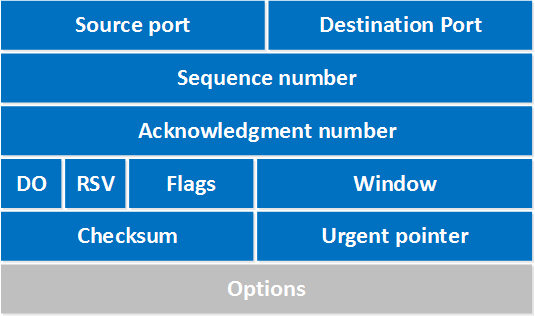
\includegraphics[width=.45\linewidth]{tcp_header.png}
        \caption{Structure of TCP packet}
    \end{subfigure}%
    ~
    \begin{subfigure}{.45\textwidth}
        \centering
        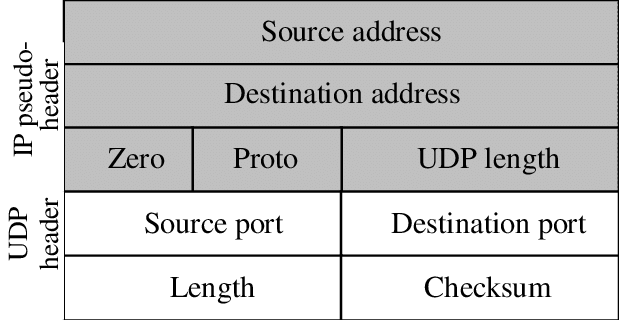
\includegraphics[width=.45\linewidth]{udp_header.png}
        \caption{Structure of UDP packet}
    \end{subfigure}
\end{figure*}

\subsection{Exploits and protection tools}

The first part of the header is part of the IP protocol.
In the second part we find different types of metadata which
are specific for the protocol. Generally the latter is redundant and such redundancy
could be exploited by a \emph{stego-algorithm}\footnote{an
algorithm used for steganography} which starting from a \emph{cover-network
packet sequence}\footnote{a sequence of packets which will be transmitted
over the network acting as a cover for the hidden messace} and a
\emph{covert message}, can generate a sequence of packets(each one embedding
a portion of the covered message) which will be sent over the network.

Despite not being \emph{risk-free} since the message could be corrupted while or even detected
while traversing the multiple nodes of the net, such procedure is widely used.

Hereinafter we illustrate a series of procedures acted at defending from this type of attacks.

\subsubsection{Tos (Type of service)}
Tos are a field in the TCP header which
are nowdays rarely used. This could open doors to a steganographic attack if
modern operating systems did not set them to zero by default.
A warden monitoring the channel could immediately signal an error.

\subsubsection{IP ID} IP ID is a field in the Internet Protocol which is used to
assist the receiver in reassemblying the fragmented packets.
This field consist of randomly unique numbers representing a packet.
It is possible to insert other types of information in this field by simply
conform to the uniqueness constraint.
Since in many cases the numbers used for the IP ID are not random, by
knowing the charachteristics of the sender it is possible to detect an
infiltration. Many networks use a \emph{Sequential Global IP ID} for network communication which uses a global counter for the
IP ID. An active warden could simply check that $IP_id2 = IP_{id1+1}$ to verify the cosistency of the message. Other systems use instead a \emph{Sequential Per-host IP ID} which is nothing but a per host sequeantial counter. 
Therefore the defence protocol is basically the same. A slightly different technique consists in the \emph{IP ID MSB Toggle} in which the \emph{OS} toggles the most significant bit of the IP ID every \emph{rekey interval}\footnote{The WPA protocol generates periodically a security key},
so that the warden can examine the MSB to check if it matches this pattern. Since the IP ID is unique, then it is common to check for non repetance of IDs.



\subsubsection{IP Fragment Offset} IP Fragment Offeset is an offset which is
present in the IP header which helps the receiver to reconstruct the sequence of
bits from the fragmented sequence.
Modulating the size of the fragments changes the offset field in the header
and thus a message could be sent.
The protection against this method is simply checking the size of the
packets relative to the MTU and so even in this case a warden can easily
detect an error.

\subsubsection{TCP sequence number} The TCP sequence number is a field in the
TCP header which stores the randomly chosen position(for security reasons) of
the first byte to be transmitted through the channel. The steganographic method
consists in replacing this field with the data to be sent.
Being random it is more difficult to spot a breach in the channel.
In this case the usage of a \emph{SVM}\footnote{Support Vector Machine}, a
machine learning tool able to identify patterns inside the data transmitted
could come into hand.
However an error could be detected even simply by checking the presence of
repetitions in the stream(not admitted by design). 

\subsubsection{Timestamp modulation} Timestamp modulation is another technique
of steganography which operate by modifing the \emph{LSB} of the timestamp of a
TCP packet in order to represent a '1'.
The covert message is thus embedded into the data stream.
Since the TCP Timestamp support is not universal, machines not supporting
such feature may detect the hidden message. Since there could be errors in the transimmssion of these packets, there is a 
threshold of randomness which must be taken into account and which could lead to some unexpected results.

\subsection{Other techniques}
There are also other methods which are simply listed(and not explained) which search for errors by checking 
\emph{unsual flags}, \emph{excessive fragmentation}, use of \emph{IP
options}, \emph{unexpected TCP options} and \emph{excessive re-ordering}.

\end{document}